\chapter{Estudo de caso: Pontos de vista sobre o governo brasileiro}
\label{estudo}
%Onde se motiva o estudo das eleições e fala pq tratará de colunas de jornalistas de notoriedade nacional. TUDO NESTE CAPÍTULO PRECISA SER BEM DIDÁTICO. FALAR DA FOLHA DILMAFACTSBYFOLHA

%mtos trabalhos de mineração de perspectiva tratam de discussão política. aproveitando o fato de que em 2010 se realizam as primeiras eleições para presidente realmente acompanhadas pela Internet, a gente decidiu fazer um estudo de caso neste assunto. Há outras pessoas pensando em coisas parecidas, como a galera do eleitorando, q criou o serviço pra fazer identificação de opinião em tweets. mas oq estamos propondo é fazer um estudo de análise das perspectivas contidas em blogs e colunas de jornalistas de notoriedade nacional, por eles serem muito lidos e contribuírem para a formação de opinião de seus leitores sobre o governo brasileiro, oq tem tudo a ver com a hora da urna. Mostre depois a estrutura da parades. fale de outros corpus e eleitorando

%Por ser um ano eleitoral, a

Muitos dos trabalhos revisados neste projeto analisam documentos que tratam de política. Em particular, boa parte deles estuda textos relacionados a governos federais - quer sejam discussões entre os próprios governantes \cite{hirst-et-al}, quer sejam artigos escritos por cidadãos ou especialistas\footnote{Todos os trabalhos mencionados nesta sentença foram revisados no Capítulo \ref{chap3}.} \cite{aaai-politics} \cite{malouf-taking_sides}. Considerando essa tendência, e o fato de que 2010 é ano de eleições para presidente no Brasil, decidiu-se realizar um estudo de caso que aproveita a abundância de artigos, disponíveis na \emph{Web}, sobre o governo Lula e a sucessão presidencial. A ideia é construir um corpus com alguns desses documentos e investigar seus pontos de vista automaticamente, classificando-os de acordo com eles e analisando, de forma subjetiva, as palavras por eles enfocadas. É válido ressaltar que não foi encontrado nenhum outro trabalho, em português, que classifique documentos de acordo com seus pontos de vista.

%Os artigos escolhidos para este estudo foram extraídos de colunas, \emph{blogs} e \emph{sites} políticos mantidos por jornalistas de notoriedade nacional. A coleta de artigos contidos em \emph{blogs} escritos por cidadãos comuns também foi cogitada - entretanto, como eles são pouco conhecidos, comentados e divulgados, essa opção exigiria um esforço de análise manual dos \emph{posts} que foge ao escopo deste projeto. Além disso, uma vantagem em focar o estudo em material publicado por jornalistas conhecidos é poder correlacionar, posteriormente, os resultados obtidos a investigações sobre a formação de opinião na mídia brasileira \emph{online} - tanto na alternativa quanto na tradicional. A seleção dos veículos para este estudo de caso resultou do consenso entre a autora desta monografia e dois jornalistas \textbf{COMO CITÁ-LOS, DIZER SEUS NOMES?}. O critério básico para as escolhas foi a defesa clara de um ponto de vista sobre o governo Lula e/ou a sucessão presidencial de 2010. 

As próximas seções deste capítulo se estruturam da seguinte forma: na seção \ref{estudo:sec1}, a construção do corpus é apresentada - desde a seleção dos veículos até a definição dos pontos de vista explorados; na seção \ref{estudo:sec2}, experimentos com um classificador Naïve Bayes\footnote{Esse classificador é apresentado no Capítulo \ref{basicos}.} são conduzidos para, assim como em outros trabalhos revisados neste projeto, se classificar artigos de acordo com seus pontos de vista; na seção \ref{estudo:sec3}, o modelo de tópicos L-LDA\footnote{Esse modelo é apresentado no Capítulo \ref{basicos}.} é aplicado ao corpus, evidenciando o uso de palavras por artigos com posicionamentos diferentes. 

% posicionamentos é analisada  
%Por serem muito lidos, e defenderem perspectivas claras nos textos que publicam, estes jornalistas têm o poder de influenciar muitos eleitores brasileiros. %análises  % mas requereria muito mais esforço de análise do que o uso exclusivo de documentos  %Lula é minha anta Dois jornalistas

\section{Construindo um corpus para estudo}
\label{estudo:sec1}

%O corpus deste estudo é composto de artigos escritos para colunas de jornais e revistas ou para \emph{sites} sobre política. São textos de caráter eminentemente opinativo, que diferem de notícias tanto pela finalidade - \textbf{blibli} - quanto pela linguagem - \textbf{blabla}. 

Os artigos escolhidos para este estudo foram extraídos de colunas, \emph{blogs} e \emph{sites} políticos mantidos por jornalistas de notoriedade nacional. A coleta de \emph{posts} de \emph{blogs} escritos por cidadãos comuns também foi cogitada - entretanto, como eles são pouco conhecidos, comentados e divulgados, essa opção exigiria um esforço de análise manual dos \emph{posts} que foge ao escopo deste projeto. Além disso, uma vantagem em focar o estudo em material publicado por jornalistas conhecidos é poder correlacionar, posteriormente, os resultados obtidos a investigações sobre a formação de opinião na mídia brasileira \emph{online} - tanto na alternativa quanto na tradicional. 

A seleção dos veículos para este estudo de caso resultou do consenso entre a autora desta monografia e os jornalistas Lucas Cunha Almeida e Andrea Duarte Bessa\footnote{Lucas Cunha, atualmente, é repórter do jornal baiano A Tarde; Andrea Bessa é gerente de comunicações da empresa Cetrel.}. O critério básico para as escolhas foi a defesa clara de um ponto de vista sobre o governo Lula e/ou a sucessão presidencial de 2010. Assim como em outros artigos revisados nesta monografia, que dividem os corpora analisados em dois lados antagônicos, assume-se que os artigos do \emph{dataset} desse estudo de caso dividem-se entre pró-situação e pró-oposição. Neste sentido, há autores que apóiam candidatos de ambos os lados, muitas vezes criticando o governo Lula e suas personalidades. Os trechos de \emph{posts} apresentados nessa seção reforçam a ideia de que essa divisão é adequada. O lado pró-situação é composto de artigos veiculados em:


%EXPLICAR Q POR SIMPLICIDADE E PQ QUASE TUDO ESTUDADO É ASSIM, DIVIDIU-SE AS PERSPECTIVAS A SEREM IDENTIF. AUTOM. EM PRÓ E ANTI GOVERNO
\begin{enumerate}

\item \textbf{Luis Nassif Online}\footnote{http://www.advivo.com.br/luisnassif/} Este é o \emph{blog} do jornalista Luis Nassif, premiado como Melhor Blog de Política pelo iBest 2008\footnote{http://idgnow.uol.com.br/internet/2008/05/21/ibest-2008-anuncia-vencedores/}. Nassif, que já trabalhou na TV Cultura e Rede Bandeirantes, mantém o \emph{blog} há cinco anos, enfocando principalmente assuntos relativos à política brasileira. Artigos do \emph{blog} são frequentemente citados, de forma positiva, em veículos de campanha pró-situação, como os \emph{sites} Blog da Dilma\footnote{http://dilma13.blogspot.com/} e Os Amigos do Presidente Lula\footnote{http://osamigosdopresidentelula.blogspot.com/}. De fato, o Luis Nassif Online adota um posicionamento pró-situação, como comprovam os trechos a seguir:

\begin{quote}
\emph{"Desde o ano passado, estava claro [sic] a falta de competitividade de José Serra, seja por não ter feito um governo brilhante em São Paulo, por não representar o novo e por não conseguir desenvolver um discurso próprio."}

{\small Retirado de \emph{"Em Minas, a mãe de todas as batalhas"} - 02/09/2010} 
\end{quote}

\begin{quote}

\emph{"Na entrevista, Bonner se limitou a perguntar da dependência de Dilma em relação à Lula [...] A consequência foi Dilma rebatendo com facilidade cada bobagem dita, reforçando o discurso social, mas sem avançar em uma proposta sequer de programa, explicando a lógica das alianças políticas. E William Bonner interrompendo-a a toda hora, impedindo sequer uma resposta completa. Algo tão desastrado e mal educado que obrigou Fátima Bernardes, do alto de sua elegância, a calá-lo com um sinal, para que parasse de ser inconveniente."}

{ \small Retirado de \emph{"O dia em que William Bonner escorregou"} - 10/08/2010}

\end{quote}

%Além de conter artigos escritos pelo próprio Luis Nassif, o \emph{blog} também publica textos de outros autores - alinhados, evidentemente, com os pontos de vista do jornalista. 

Como o veículo possui muito conteúdo, foram considerados apenas os artigos da categoria "Eleições".  

\item \textbf{Conversa Afiada}\footnote{http://www.conversaafiada.com.br/} O \emph{site} se define como um portal de jornalismo independente, contendo principalmente artigos produzidos por Paulo Henrique Amorim. O jornalista, que já trabalhou para as Redes Globo e Bandeirantes e para a revista Carta Capital, mantém o \emph{site} desde 2006. Enfocando a política brasileira, o Conversa Afiada apóia, dentre outras iniciativas do governo federal, a candidatura da ex-ministra Dilma Rousseff\footnote{http://www.conversaafiada.com.br/brasil/2010/07/02/mino-explica-por-que-apoia-a-dilma-porque-ela-e-melhor-que-o-serra/}. Os trechos abaixo justificam a escolha do \emph{site} como representante da mídia \emph{online} pró-situação:

\begin{quote}

\emph{"O Governo Lula é um sucesso e a popularidade dele, recordista desde o primeiro dia de Governo. Promoveu a inclusão social, ampliou a classe média e assistiu os pobres. Fez uma política externa que não tirou o sapato para os Estados Unidos. A Dilma é a sua legítima sucessora: foi a CEO do Governo Lula. O Serra é um nada."}

{\small Retirado de \emph{"A Dilma não é um tsunami. Dilma é o rio que segue para o mar"} - 27/08/2010}
\end{quote}

\begin{quote}

\emph{"Segundo a tevê DEMO-Tucana da Bahia, a afiliada da Globo, Jacques Wagner está na frente de Paulo Souto por 46\% a 19\%. Paulo Souto é o aliado de Serra na Bahia. A TV Bahia, também."}

{\small Retirado de \emph{"Sumiram com o dinheiro do Serra. Serra é barrado em procissão"} - 07/08/2010}
\end{quote}

%Os artigos do \emph{site} muitas vezes citam notícias retiradas de portais, como o G1 ou UOL, a fim de contextualizar críticas e análises.

Também por possuir muito conteúdo, apenas os artigos pertencentes à categoria "Política" foram considerados.
% Prêmio iBest de Melhor Blog de Política, em eleição popular e da Academia iBest. 

\item \textbf{Escrevinhador}\footnote{http://www.rodrigovianna.com.br/} O \emph{blog}, mantido pelo \emph{site} da revista Caros Amigos, é escrito pelo jornalista Rodrigo Vianna, que também é repórter da Rede Record. Ele está no ar desde 2008, enfocando acontecimentos da vida política do Brasil e do Mundo. No que diz respeito ao Brasil, o conteúdo do \emph{blog} assume uma perspectiva pró-situação, como ilustram os trechos abaixo:

\begin{quote}

\emph{"Abandonado pelos aliados do DEM e do PSDB, em queda nas pesquisas, Serra refugia-se na mídia. O candidato do PSDB virou isso: porta-voz dos interesses da velha mídia. Faz sentido. É quem, em última instância, sustenta a candidatura."}

{\small Retirado de \emph{"Serra, porta-voz da velha mídia; é Zé ou Mané?"} - 19/08/2010}
\end{quote}

\begin{quote}
\emph{"O programa da Dilma foi um show. [...] Foi um programa em que Lula não apareceu mais que Dilma, e nem sumiu – porque seria falso, ela é a candidata dele. Foi um programa em que Lula passou o bastão a Dilma. De forma eficiente, corajosa e, ao mesmo tempo, emocionante."}

{\small Retirado de \emph{"Dilma acerta a mão; Serra quer virar 'Zé'"} - 18/08/2010}

\end{quote}

Como o \emph{blog} também trata de outros assuntos, apenas as categorias "Plenos Poderes" e "Palavra Minha", mais direcionadas à política, foram consideradas para extração de artigos.

\item \textbf{Brasília, eu vi}\footnote{http://brasiliaeuvi.wordpress.com/} O \emph{blog}, escrito pelo jornalista Leandro Fortes, que também trabalha para a revista Carta Capital, agrega alguns de seus artigos para a revista e outros textos sobre política. Estes artigos têm boa recepção em \emph{sites} de campanha pró-situação, como o Blog da Dilma\footnote{http://dilma13.blogspot.com/2010/08/caso-lunus-verdade-dos-fatos.html}. De fato, eles assumem uma perspectiva de defesa da situação, como justificam os trechos abaixo:


\begin{quote}
\emph{"Assim, enquanto a imprensa mundial se dedica a decodificar as engrenagens e circunstâncias que fizeram de Lula o mais importante líder mundial desse final de década, a imprensa brasileira se debate em como destituí-lo de toda glória, de reduzí-lo a um analfabeto funcional premiado pela sorte, a um manipulador de massas movido por programas de bolsas e incentivos [...]."}

{\small Retirado de \emph{"Não verás Lula nenhum"} - 18/05/2010}
\end{quote}

\begin{quote}

\emph{"Ao acusar o presidente Luiz Inácio Lula da Silva de ter transformado o Brasil em uma “república sindicalista”, José Serra optou por agregar a seu modelito eleitoral, definitivamente, o discurso udenista de origem, de forma literal, da maneira como foi concebido pelas elites brasileiras antes do golpe militar de 1964."}

{\small Retirado de \emph{"Serra precisa de mais amigos"} - 15/07/2010}
\end{quote}
\end{enumerate}


O lado pró-oposição, por sua vez, é composto de artigos veiculados em:

\begin{enumerate}

\item \textbf{Reinaldo Azevedo}\footnote{http://veja.abril.com.br/blog/reinaldo/} O \emph{blog}, escrito pelo jornalista homônimo, é mantido pela revista Veja. Autor da frase \emph{"Tudo que é bom para o PT é ruim para o Brasil"} \cite{bom-pt-mau-brasil}, Reinaldo Azevedo, que já foi editor da Folha de S. Paulo, alimenta seu \emph{blog} com críticas ao governo atual, como evidenciam os trechos abaixo:

\begin{quote}

\emph{"O problema dos petistas é que eles são viciados no aulicismo, na cortesania. Ao conviver com pessoas que sempre têm um preço, ficam chocados e tomam como ofensa pessoal a descoberta de que nem todos se comportam com essa moral anã."}

{\small Retirado de \emph{"Presidente do PT repete ladainha autoritária do programa 'Rubriquei, mas não traguei'. Ou: 'Ai que vontade de censurar a Veja!!!' Contenha a coceira, companheiro!} - 15/07/2010} 
\end{quote}

\begin{quote}

\emph{"Cinco centrais sindicais assinaram um vergonhoso manifesto contra a candidatura do tucano José Serra à Presidência. Antes de mais nada, e a despeito da mentira essencial que está contida no texto — já falo a respeito —, cumpre destacar: trata-se de um manifesto ilegal, de mais um crime eleitoral escancarado."}

{\small Retirado de \emph{"Acuado pelo 'Rubriquei, mas não traguei', PT mobiliza centrais sindicais. E elas assinam um documento ilegal e mentiroso."} - 12/07/2010 }

\end{quote}

\item \textbf{Coluna do Augusto Nunes}\footnote{http://veja.abril.com.br/blog/augusto-nunes/} A coluna, parte da revista Veja, é escrita pelo jornalista Augusto Nunes, que também apresenta o programa Roda Viva na TV Cultura. Seus artigos têm má recepção em alguns veículos que defendem o atual governo, como o Luis Nassif Online\footnote{http://www.advivo.com.br/blog/luisnassif/serra-e-fhc-uma-relacao-delicada} e o Blog da Dilma\footnote{http://dilma13.blogspot.com/2010/01/mais-uma-do-tucano-augusto-nunes.html}, justamente por assumirem uma posição pró-oposição. Os trechos abaixo justificam esta perspectiva:


\begin{quote}

\emph{"Como todo sinal de alarme, o som de um neurônio em ebulição é  perturbador, mas muito útil. Quem tem juízo entenderá que Dilma Rousseff não é uma candidata em campanha. É uma ameaça a caminho."}

{\small Retirado de \emph{"O som perturbador do neurônio em ebulição"} - 20/07/2010}

\end{quote}

\begin{quote}

\emph{"O eleitor merece saber se Lula recebeu uma herança maldita e reconstruiu o país, como repete há pelo menos seis anos, ou se resolveu valer-se de mentiras e fantasias para desqualificar o legado do antecessor que acabou com a inflação, consolidou a democracia constitucional e fixou diretrizes econômicas que, em sua essência, vigoram até hoje."}

{\small Retirado de \emph{"FHC aceita o convite para o duelo que Lula não pode recusar."} - 11/02/2010}
\end{quote}

Todos os artigos extraídos dessa coluna pertencem à categoria "Direto ao Ponto", por ela tratar especificamente da política brasileira atual.

\item \textbf{Coluna do Diogo Mainardi}\footnote{http://veja.abril.com.br/blog/mainardi/} A coluna, escrita desde 2002, é a mais lida da revista Veja segundo ela mesma, reunindo críticas à política e à economia brasileiras. O jornalista Diogo Mainardi se opõe aos governos petistas, tendo inclusive publicado, em 2007, o livro Lula é Minha Anta \cite{lula-anta}, no qual agrupa diversos artigos escritos para sua coluna na Veja. Os trechos abaixo ilustram a posição de Mainardi como um grande crítico do governo do PT e de sua candidata Dilma Rousseff:

\begin{quote}

\emph{"Dilma Rousseff teve uma loja de produtos importados. O empreendimento durou menos de um ano e meio. Se Dilma Rousseff mostrar como presidente da República o mesmo talento que mostrou como empresária, o Brasil já pode ir fechando as portas."}

{\small Retirado de \emph{"Dilma 1,99 Rousseff"} - 04/09/2010}
\end{quote}  

\begin{quote}

\emph{"No futuro, quando alguém quiser relatar os fatos deste período, terá de recorrer necessariamente aos processos judiciais, que detalharam o modo lulista de se organizar, de se acumpliciar, de se infiltrar e de fazer negócios."}

{\small Retirado de \emph{"A história em inquéritos"} - 20/03/2010}
\end{quote}

\item \textbf{Portal de Carlos Alberto Sardenberg}\footnote{http://www.sardenberg.com.br/site/index.php} O portal contém artigos do jornalista para suas colunas nos jornais O Globo e O Estado de S. Paulo, além de outros textos de análise política e econômica. Além destas ocupações, Sardenberg também é comentarista da TV Globo e âncora da Rádio CBN, tecendo comentários sobre a economia mundial e brasileira. Os trechos abaixo transparecem seu posicionamento pró-oposição: 

\begin{quote}

\emph{"O governo Lula não quer fazer concessões à iniciativa privada porque está num ímpeto estatizante, em ano eleitoral. Só que o Estado não tem os recursos para fazer nada de substancial. Fica por isso mesmo."}

{\small Retirado de \emph{"As tarefas de Lula"} - 22/03/2010}
\end{quote}

\begin{quote}

\emph{"É verdade que o país está de novo em um bom momento. Mas não é verdadeira a conclusão que o 'lulismo' tira disso: que isso tudo só está acontecendo porque Lula é o presidente."}

{\small Retirado de \emph{"A salvação?"} - 01/04/2010}
\end{quote}
\end{enumerate}

É válido ressaltar que os autores dos artigos muitas vezes colocam trechos de notícias, ou mesmo textos críticos de outros autores, em seus escritos, colaborando para a riqueza da linguagem no corpus.

Outros veículos foram cogitados, como o Blog do Noblat\footnote{http://oglobo.globo.com/pais/noblat/}, o \emph{blog} de Miriam Leitão para o jornal O Globo\footnote{oglobo.globo.com/economia/miriam/}, a coluna de Cristiana Lôbo para o portal G1\footnote{http://g1.globo.com/platb/cristianalobo/} e o \emph{blog} de Celso Ming para o jornal O Estado de S. Paulo\footnote{blogs.estadao.com.br/celso-ming/ }. Os posicionamentos contidos nestes veículos, entretanto, não foram considerados claros o suficiente para os propósitos deste estudo. 

Todos os artigos contidos nas colunas, \emph{sites} e \emph{blogs} selecionados foram  publicados entre 01/01/2010 e 06/09/2010. O período fixado, por fazer parte de um ano eleitoral, encerra uma quantidade significativa de artigos pró-situação e pró-oposição. Por este motivo, e também para manter o escopo do estudo atrelado às eleições 2010, artigos de anos anteriores não foram coletados. A extração dos documentos foi feita de forma automatizada com \emph{scripts} desenvolvidos nas linguagens de programação Python\footnote{http://python.org/} e UNIX ShellScript\footnote{http://www.gnu.org/software/bash/manual/bashref.html}. Todos eles estão disponíveis no repositório \emph{online} de Aline Bessa\footnote{http://github.com/alibezz}. Como os jornalistas eventualmente publicam sobre política mundial ou outros assuntos, foi feita uma filtragem nos artigos, de modo a restarem apenas aqueles que contêm pelo menos uma das seguintes palavras-chave: "Lula", "FHC", "Dilma", "Serra", "Marina", "PT", "PV", "PSDB". Todos os documentos foram, por fim, anonimizados, para que os nomes de seus autores não interferissem nos estudos. 

Após filtragem e anonimização, restaram 1065 artigos pró-situação e 2747 pró-oposição. Para os estudos feitos com o corpus, envolvendo o classificador Naïve Bayes e o modelo de tópicos L-LDA, reduziu-se a quantidade de documentos pró-oposição para 1065, utilizando-se apenas 550 dos 2377 artigos extraídos do \emph{blog} de Reinaldo Azevedo, amostrados aleatoriamente. Essa estratégia foi adotada porque o classificador se mostrou sensível a quantidades muito discrepantes de palavras por ponto de vista. Como o uso do L-LDA estende as análises feitas com o classificador, decidiu-se manter o corpus idêntico para ambos os estudos. 

\begin{table}[t]
\centering
\begin{tabular}{| l | l | p{5cm} | }
\hline

\textbf{Veículo} & \textbf{Coleta} & \textbf{Filtragem/Anonimização} \\ \hline

\textbf{Reinaldo Azevedo} & 2490 & 2377\ensuremath{^*} \\ \hline
\textbf{Augusto Nunes} & 579 & 450 \\ \hline
\textbf{Diogo Mainardi} & 40 & 32 \\ \hline
\textbf{Carlos Sardenberg} & 59 & 33  \\ \hline
\textbf{Conversa Afiada} & 375 & 337  \\ \hline
\textbf{Luis Nassif Online} & 994 & 525 \\ \hline
\textbf{Escrevinhador} & 222 & 179  \\ \hline
\textbf{Brasília, eu vi} & 34 & 24  \\ \hline
\end{tabular}
\label{tab1:estudo}
\caption{Quantidades de artigos disponíveis em cada etapa da construção do corpus. \ensuremath{^*}Apenas 550, amostrados aleatoriamente, foram aproveitados.}
\end{table}

O número de artigos coletados em cada veículo varia bastante, como pode ser observado na Tabela 4.1. No corpus sobre o conflito Israel-Palestina, estudado por Lin et al. em trabalho revisado no Capítulo \ref{chap3}, este comportamento também foi observado. Os documentos desse \emph{dataset} foram escritos por diversos autores, e alguns deles contribuíram com muito mais textos do que outros. Ainda assim, como pode ser verificado na revisão apresentada no Capítulo \ref{chap3}, os resultados obtidos são de alta qualidade \cite{lin-et-al2006}. Isto reforça a ideia de que essa variação não interfere significativamente na qualidade dos experimentos feitos com o corpus deste estudo de caso.


\section{Classificando documentos com um Naïve Bayes}
\label{estudo:sec2}

O primeiro estudo conduzido com esse corpus consiste na classificação dos artigos de acordo com os pontos de vista pró-oposição e pró-situação. Esse capítulo não se propõe a comparar classificadores diferentes, de modo que o Naïve Bayes será a única técnica explorada em seu escopo. O classificador Naïve Bayes foi escolhido porque, de acordo com a revisão do Capítulo \ref{chap3}, não há um consenso sobre qual dos dois - ele ou um SVM - é mais indicado para classificação por ponto de vista. Em alguns trabalhos o Naïve Bayes conduz a melhores resultados; em outros, o SVM. Essas questões, e a consideração de que o Naïve Bayes é mais simples de implementar, justificam sua escolha.  

O classificador explora apenas as contagens de palavras dos documentos para definir suas classes. Os motivos para essa escolha foram: popularidade do uso nos trabalhos revisados no Capítulo \ref{chap3}, o que indica essa escolha como a mais natural; simplicidade de computação, dado que essa escolha envolve apenas a soma das ocorrências de palavras; fácil adaptação a qualquer língua, em particular a portuguesa. 

% por contagens de palavras também são os mesmos apontados no Capítulo \ref{chap3}, na seção \ref{freqs:experim}. 

Essas escolhas se mostraram adequadas para o problema: a taxa de acerto obtida na classificação foi de 89.43\%. Assim como em outros artigos revisados no Capítulo \ref{chap3} \cite{lin-et-al2006, aaai-politics, klebanov}, esse valor foi obtido via validação cruzada por dez vezes\footnote{Essa técnica de validação é apresentada no Capítulo \ref{basicos}.}. Ou seja, ele corresponde à média aritmética das taxas de acerto obtidas via essa forma de validação. De modo semelhante, a precisão, recuperação e métrica F1\footnote{Essas métricas são descritas no Capítulo \ref{basicos}.}  associadas a cada classe (ponto de vista) foram obtidas, e constam na Tabela 4.2. %tabela mais precisa %precisao 0 0,915979712 precisao 1 0,877579312 % recuperação 0 0,870754717 1 0,917924528  %f1 0 0,891837888 1 0,896484354

%; a precisão média, de  89.68\%; a métrica F1 média, de 89.42\%

\begin{table}[h]
\centering
\begin{tabular}{| l | l | l | l | }
\hline

\textbf{Classe} & \textbf{Precisão} & \textbf{Recuperação} & \textbf{Métrica F1} \\ \hline

\textbf{Pró-situação} & 91.60\% & 87.08\% & 89.18\% \\ \hline
\textbf{Pró-oposição} & 87.78\% & 91.79\% & 89.65\% \\ \hline
\end{tabular}
\label{resultados}
\caption{Métricas de desempenho associadas a cada classe.}
\end{table}

A primeira coluna da Tabela 4.2 indica que o Naïve Bayes classificou menos documentos erroneamente como pró-situação do que como pró-oposição. Em outras palavras, a classificação como pró-situação foi mais precisa. A segunda coluna indica que, por outro lado, o Naïve Bayes classificou mais documentos pró-oposição corretamente. Neste sentido, a recuperação funciona como a taxa de acerto. Por fim, a terceira coluna indica que, ponderando as colunas anteriores via métrica F1, os resultados obtidos são praticamente idênticos. Isso significa, na prática, que o Naïve Bayes apresenta um desempenho bastante equilibrado considerando-se ambas as classes. 

O bom desempenho obtido com o Naïve Bayes indica que o uso de metodologias mais complexas, envolvendo aspectos sintáticos dos documentos, por exemplo, não é necessário. Além disso, é válido ressaltar que a adoção de características sintáticas/semânticas, para a classificação de um corpus em português, não é tão simples como para um corpus em inglês. Isso advém  da carência de \emph{softwares} e dicionários semânticos para a língua portuguesa - em particular, a variação utilizada no Brasil. Esses \emph{softwares} e dicionários colaboram com a determinação de diversos aspectos gramaticais/linguísticos dos textos, minimizando o esforço manual requerido quando eles não podem ser utilizados.


Os valores obtidos com o classificador Naïve Bayes são comparáveis àqueles obtidos por \textbf{Durant e Smith} em seu trabalho sobre George W. Bush e a Guerra do Iraque\footnote{Esse trabalho foi revisado no Capítulo \ref{chap3}.} \cite{durant-smith}: 89.77\%. É válido ressaltar que, diferentemente da metodologia adotada por Durant e Smith, nenhuma palavra foi descartada no processamento dos textos para este estudo de caso.  

Os artigos escolhidos para este corpus são compostos, muitas vezes, de textos de outros autores. Isto reforça a ideia de que o classificador Naïve Bayes está efetivamente aprendendo os pontos de vista dos documentos, em vez de estilos de escrita. De todo modo, assim como no estudo de \textbf{Lin et al.} sobre o conflito Israel-Palestina\footnote{Esse trabalho foi revisado no Capítulo \ref{chap3}.} \cite{lin-et-al2006}, foi conduzido um experimento em que os artigos pertencentes aos conjuntos de treinamento e teste são escritos por autores diferentes. Se o que está sendo aprendido são de fato os pontos de vista dos documentos, o desempenho do classificador não deve ser muito diferente do obtido na validação cruzada por dez vezes. Testando com artigos da coluna de Augusto Nunes e do \emph{site} Conversa Afiada, e treinando com os demais, a taxa de acerto obtida foi de 92.79\%, acompanhada de precisão média de 93.32\% e métrica F1 média de 91.86\%. Este experimento, portanto, ratifica os outros resultados, evidenciando que o classificador Naïve Bayes cumpre bem a tarefa de identificar os pontos de vista pró-oposição e pró-situação.

% indicado para identificar perspectivas em artigos opinativos.
%Uma alta taxa de acerto também indica que a identificação de perspectiva política em \emph{blogs} brasileiros, cujas linguagens se assemelham às estudadas, pode apresentar um bom resultado.

%Se a taxa de acerto for alta, é possível pensar em aplicações que envolvam a identificação da perspectiva d


%- talvez até escritas por blogueiros comuns, em vez de jornalistas.


\section{Ilustrando o uso de palavras por ponto de vista}
\label{estudo:sec3}
%Onde se explica o uso do L-LDA, o overlap de palavras, mostra-se snippets e talz.

A análise das principais palavras enfocadas por cada ponto de vista amplia a compreensão dos resultados obtidos na seção anterior. A alta taxa de acerto obtida sugere que os jornalistas se expressam de forma bastante diferente, de modo que o Naïve Bayes não \emph{se engana} com muita frequência. Em outras palavras, como essas expressões foram quantificadas via contagens de palavras, a alta taxa de acerto indica que essas características foram suficientes para discrimar documentos de classes diferentes. Essa seção se propõe a ilustrar quais palavras foram mais destacadas por eles, colaborando para a transmissão de pontos de vista diferentes.

Para a investigação sobre essas palavras, foi feita uma aplicação do modelo L-LDA. Cada documento foi associado a dois tópicos: um neutro, igual para todos eles, e um referente a seu ponto de vista (pró-oposição ou pró-situação). Há, portanto, três tópicos diferentes nesta aplicação. O uso de um tópico neutro, associado a todos os documentos, ajuda a filtrar palavras muito comuns nos \emph{datasets}, independentemente de ponto de vista. Dois exemplos são as palavras \emph{vez} e \emph{campanha}. Essa é a diferença fundamental entre essa aplicação do L-LDA e a simples contagem de palavras em documentos, dividida entre os dois pontos de vista. Esse tipo de contagem não diferencia quais palavras são \emph{mais destacadas} em documentos escritos sob uma certa perspectiva e quais são \emph{muito utilizadas} por todos eles. Essas últimas possivelmente não os discriminam tanto quanto as primeiras.

% Cada documento de ambos os \emph{datasets} foi associado a dois tópicos: um neutro, idêntico para todos eles, e outro referente a seu ponto de vista. No primeiro corpus, esses pontos de vista são pró-Israel ou pró-Palestina; no segundo, republicano ou democrata. Há portanto, em cada corpus, três tópicos diferentes.


%O motivo para isso é  que a classificação em si se baseia nesses usos de palavras, através de suas contagens. Neste sentido, portanto, a compreensão de quais palavras receberam mais destaque 

% o modelo generativo L-LDA foi aplicado ao corpus. Cada artigo O uso desses tópicos evidencia quais palavras são mais enfocadas por cada ponto de vista. % e quais são utilizadas de forma muito semelhante em todo o corpus (genérico).

%Para a investigação sobre o uso de palavras,
A Tabela 4.3 elenca as dez palavras mais frequentemente associadas a cada ponto de vista. O tópico neutro não será analisado, haja vista que foi utilizado apenas para auxiliar na filtragem das palavras mais comuns do corpus. Em alguns casos, essas palavras coincidem nos dois pontos de vista. Isso significa que ambos deram muito destaque a elas.

%em dois ou mais tópicos. Se o genérico não estiver presente, i

%essa palavra. Em caso contrário, tem-se que a palavra, além de ser muito enfocada por pelo menos uma das duas perspectivas, é também uma das mais comuns no corpus.

\begin{table}[h]
\centering
\begin{tabular}{| l | p{10cm} | }
\hline
\textbf{Tópico} & \textbf{Palavras} \\ \hline
\textbf{Pró-situação} & serra, dilma, lula, psdb, presidente, pt, candidato, folha, tucano, eleições\\ \hline
\textbf{Pró-oposição} & dilma, lula, presidente, brasil, rousseff, pt, gente, candidata, mundo, candidato \\ \hline
\end{tabular}
\label{tab:palavras}
\caption{As dez palavras mais frequentemente associadas aos tópicos pró-situação e pró-oposição, em ordem e excluindo-se artigos, preposições, conjunções, advérbios e pronomes pessoais.}
\end{table}

%\textbf{Genérico} &  governo, brasil, serra, estado, lula, poder, presidente, nacional, vez, campanha \\ \hline

%JUSTIFICAR ISSO DIREITO, E FAZER AS FIGURAS
A Tabela 4.3 indica que as palavras enfocadas por pontos de vista diferentes são as mesmas em alguns casos, diferindo apenas na forma como são enfatizadas. Em outras palavras, a ordem das palavras nessa tabela corresponde, diretamente, ao quanto elas se associaram a cada tópico. Os artigos pró-oposição, por exemplo, dão muito destaque às palavras \emph{lula} e \emph{dilma}; os pró-situação, por sua vez, também enfatizam estas palavras, mas dão um destaque maior a \emph{serra}, candidato à presidência pelo PSDB. A associação de palavras semelhantes aos tópicos pró-oposição e pró-situação advém do fato de que os artigos compartilham um tema geral - o governo brasileiro - e, consequentemente, o mesmo vocabulário básico. É diferente do que acontece quando os tópicos correspondem a temas diferentes em vez de pontos de vista, como pode ser visto no trabalho de Ramage et al. sobre \emph{tags} de \emph{blogs} \cite{llda}.

Para visualizar melhor a ênfase dada às palavras na Tabela 4.3, elas foram processadas pelo \emph{software} wordle\footnote{http://wordle.net}, resultando nas figuras \ref{situacao} e \ref{oposicao}. O tamanho das palavras nas imagens está relacionado ao número de vezes que elas se associam a cada tópico. As imagens evidenciam o destaque dado aos políticos Lula, Dilma Rousseff e José Serra nos artigos analisados. %A imagem \ref{generico} dá certo destaque a Lula e José Serra, mas também enfatiza outros termos, como \emph{governo} e \emph{brasil}, relacionados mais genericamente à temática dos artigos: a política brasileira.

%Isso fica mais claro nas Figuras \ref{situacao} e \ref{oposicao}. É válido ressaltar que, nos experimentos do Capítulo \ref{chap3}, foram geradas imagens como essas, mas elas não indicaram ênfases muito diferentes no uso das palavras selecionadas.
\begin{figure}[h]
  \centering % este comando é usado para centralizar a Figura
  
\includegraphics[width=12.5cm, height=5cm]{situacao.png}\\
  \caption{Representação gráfica para as dez palavras associadas ao tópico pró-situação na Tabela 4.3.}
  \label{situacao}
\end{figure}

\begin{figure}[h]
  \centering % este comando é usado para centralizar a Figura
  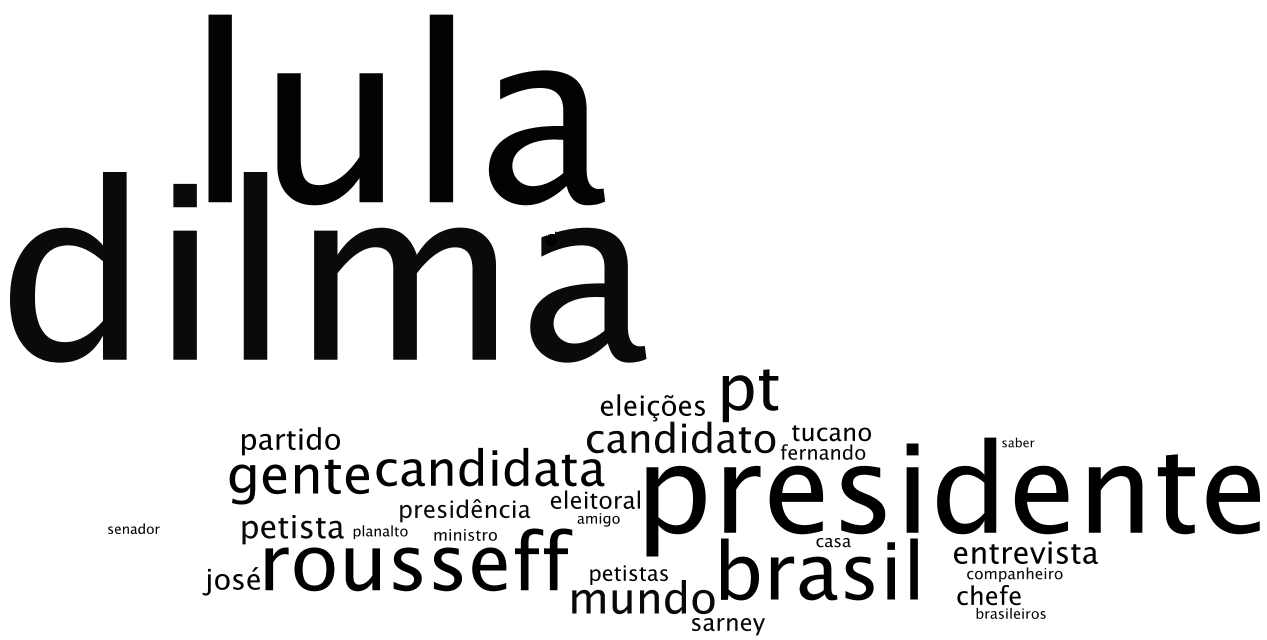
\includegraphics[width=11.5cm, height=6.5cm]{oposicao.png}\\
  \caption{Representação gráfica para as dez palavras associadas ao tópico pró-oposição na Tabela 4.3.}
  \label{oposicao}
\end{figure}



%\begin{figure}[h]
%  \centering % este comando é usado para centralizar a Figura
%  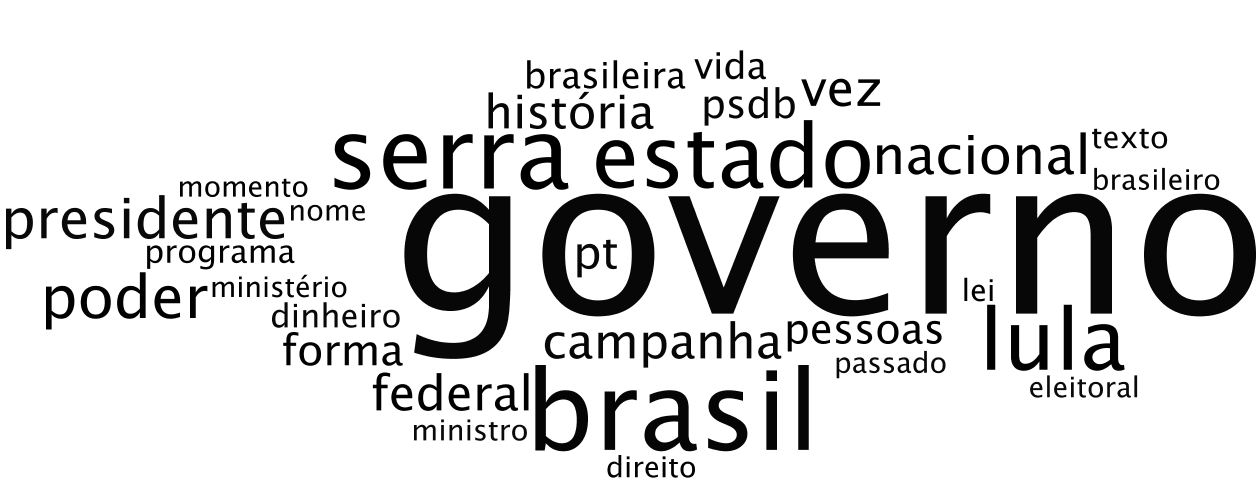
\includegraphics[width=12.5cm, height=6.5cm]{generico.png}\\
%  \caption{Representação gráfica para as dez palavras associadas ao tópico genérico na Tabela 4.3.}
%  \label{generico}
%\end{figure}

Essas figuras também sugerem que os artigos pró-situação dão mais enfoque a personalidades relacionadas à situação, como Lula e Dilma Rousseff, do que os pró-oposição a personalidades da oposição, como José Serra ou Marina Silva. Essa última, inclusive, candidata à presidência pelo PV, não foi mencionada nas palavras listadas na Tabela 4.3. Essas duas observações evidenciam que os veículos, no período analisado, concentraram seus antagonismos em personalidades políticas dos partidos PT, como Lula e Dilma Rousseff, e PSDB, como José Serra. 

%É válido ressaltar, por fim, que, apesar dos textos terem caráter crítico e não necessariamente informativo, as palavras elencadas na Tabela 4.3 não carregam uma polaridade natural, como no caso dos adjetivos \emph{bom} ou \emph{ruim}. Isso reforça a ideia de que a expressão de pontos de vista não é tão simples quanto a emissão de opiniões pontuais e claramente polarizadas, como \emph{Serra é um candidato ruim} ou \emph{Lula é um presidente bom}. 

Os pontos de vista desse corpus são construídos através de argumentações complexas, como indicam os trechos de artigos apresentados na seção \ref{estudo:sec1}. Para compreender melhor a relação que as palavras da Tabela 4.3 estabelecem com eles, recomenda-se, por fim, a leitura de um número razoável de passagens de texto que as contenham. Alguns trechos foram selecionados abaixo, em caráter ilustrativo:

\begin{quote}
\emph{"O que parece estarrecedor para quem nunca ouviu \textbf{Dilma} antes - e tenho colegas jornalistas que nunca a viram discursando ou dando \textbf{entrevista} - é absolutamente familiar para os frequentadores desta coluna. Que há nove meses têm acesso a veementes indícios, há muito transformados em provas documentais, de que \textbf{Dilma} é uma afronta imposta ao \textbf{Brasil} por \textbf{Lula}, num [sic] crime lesa-pátria sem perdão."}

{\small Retirado de "O som perturbador do neurônio em ebulição", da coluna de Augusto Nunes - 20/07/2010}
\end{quote}

\begin{quote}
\emph{"Que o \textbf{tucano} \textbf{José} Serra se saiu muito melhor no \textbf{Jornal} Nacional e que a eleição é, sim, de continuidade — no sentido de que não cabe mais falar em ruptura. E fiz uma crítica ou outra ao governo \textbf{Lula}."}

{\small Retirado de "A cabeça dos brasileiros... autoritários", do \emph{blog} de Reinaldo Azevedo - 15/08/2010}
\end{quote}

\begin{quote}

\emph{"A última bala na agulha do \textbf{Serra} é a baixaria. Só que, na era da internet, a baixaria – Lunus (para desconstruir Roseana Sarney) e aloprados do \textbf{PT} (para mandar as ambulâncias superfaturadas para o Inferno) – não tem o mesmo efeito do passado.É o caso dos aloprados do tal dossiê que ele vai ter que explicar na Justiça."}

{\small Retirado de "Serra só tem uma saída: pendurar FHC no pescoço", do \emph{site} Conversa Afiada - 07/06/2010}
\end{quote}

\begin{quote}
\emph{"A entrevista de \textbf{Dilma} ao JN foi didática: \textbf{Dilma} conseguiu colar sua \textbf{candidatura} como continuidade das políticas do governo \textbf{Lula}. Ponto pra ela.Por outro lado, o casal número um do JN da \textbf{Globo} escorregou e mostrou claramente contra quem trabalham em 2010 e a favor de quem se esforçam para mudar tudo o que está aí."}

{\small Retirado de "O povo não é (mais) bobo...", do \emph{blog} Luis Nassif Online - 10/08/2010}
\end{quote}


